\chapter{Theory and Background}

\section{The Semiconductor Quantum Well}
\subsection{The Bandgap}
\indent In order to understand the state of electrons in a crystalline solid, one must first understand the problem of how electrons act under the effect of a periodic charge density. The Bloch theorem is a useful tool for understanding this problem quantum-mechanically, and a complete treatment can be found in CITE Iadonisi. Here, I will sketch the important physical concepts and their implications for my thesis. Consider an infinite, arbitrary crystalline atomic lattice, unbounded in each spatial direction. The crystalline structure, therefore, is homogeneous, uniform, and evidently invariant under translation along any of the crystalline axes. Thus, for each valance electron around an arbitrary lattice atom, the following is true:

\begin{equation}
H(\vec{r}) = H(\vec{r} + \vec{D_n})
\end{equation}

where $\vec{r}$ is an arbitrary lattice position and $\vec{D_n}$ is an arbitrary displacement from position $\vec{r}$ and $H(\vec{r})$ is the quantum-mechanical Hamiltonian for a lattice electron. We can thus define a lattice transition operator, $T_n$, which takes the electron wavefucntion at one lattice site and spits out an electron wave function for a chosen $D_n$.

\begin{equation}
T_n \ket{\psi(\vec{r})}=\ket{ \psi(\vec{r} + \vec{D_n})}
\end{equation}

Because our operator commutes with itself and the Hamiltonian, we can assume that $T_n$ and $H$ share the same eigenfunctions. Thus the following vector equation holds:

\begin{equation}
T_n\ket{\psi(\vec{r})} = c_n(\vec{D_n})\ket{\psi(\vec{r} + \vec{D_n})}
\end{equation}

where the $c_n(\vec{D_n})$ coefficients are the eigenvalues of $T_n$. The wave function \textit{must} remain normalized through some arbitrary displacement $\vec{D_n}$, and we can thus choose:

\begin{equation}
c_n(\vec{D_n}) = e^{i \vec{k} \cdot \vec{D_n}}
\end{equation}
where $\vec{k}$ is the electron's wave vector (real, unless translational symmetry is broken). We can then write the Bloch theorem:

\begin{equation}
T_n \ket{ \psi(\vec{r})} = e^{i\vec{k} \cdot \vec{D_n}} \ket{\psi(\vec{r})}
\end{equation}
where $\ket{\psi(\vec{r})} = e^{i\vec{k} \cdot \vec{D_n}}\ket{u_k(\vec{r})}$ is the Bloch wave function, and $u_k(\vec(r))$ is a periodic function of the lattice. We can then write out the full Shr\"{o}dinger equation for an electron in our arbitrary lattice, after substitution of our Bloch wavefunctions:
\begin{equation}
\Big (-\frac{ \hbar ^2}{2m} \bigtriangledown ^2 - \frac{ i\hbar^2}{m} \vec{k} \cdot \bigtriangledown + \frac{\hbar^2 k^2}{2m} + V \Big )\ket{u_k} = E \ket{u_k}
\end{equation}

\indent Solving this equation is far beyond the scope of the thesis, but the upshot is that in a periodic lattice (i.e. a periodic charge distribution establishes periodic boundary conditions), allowed energy states smear into allowed `bands'. Crudely, electrons can occupy the `conduction band' states where they are free to move about the lattice structure. They are otherwise confined to their host atoms and occupy the `valance band' states. The energy difference between the valance band and conduction band is called the bandgap, and is illustrated in the dispersion curve, \ref{Example band structure of a direct-gap semiconductor.}. 

\begin{figure}[h!]
\centering
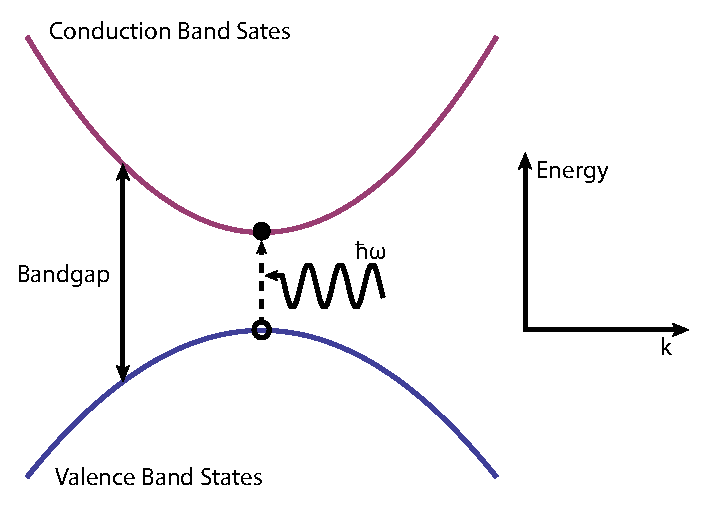
\includegraphics[width = .8\textwidth]{dispcurve.eps}
\caption{A typical dispersion curve minima for a direct-gap semiconductor. An optical transition is illustrated at $\vec{k} = 0$, where an electron is emitting a photon as the result of a transition from the conduction band to the valance band.}
\label{Example band structure of a direct-gap semiconductor.}
\end{figure}

\indent The full functional shape of dispersion curves is dependent on the physical properties of solids. Thus, solids can be broadly construed into three categories: metals, insulators, and semiconductors. In metals, the conduction band energies are below the Fermi level and thus some electrons are free to move about and conduct charge. In insulators, the bandgap is relatively large, and therefore electrons are confined to their host atoms. By contrast in semiconductors, the bandgap is fairly small and therefore only a small amount of energy is required to promote an electron to the conduction band from the valance band. Importantly, semiconductor electrons can be optically photo-excited into the conduction band. This fact forms the basis of experimental studies of semiconductor nanostructure CITE Steve, photonic devices, and certain types of theoretical quantum information processing schemes CITE Nature Review of QI.

\subsection{Confinement and The Exciton}

\indent It is well known that nanometer scale confinement of particles results in quantized energy states CITE someone. I'll illustrate the important physical effects of confinement, and in the next section, I will introduce the semiconductor quantum well. Initially, I will sketch the derivation of the finite potential well that confined particles feel. This derivation will be sufficient to explore the physical effects of confinement, but the subtleties of the semiconductor electron potential will be addressed in the next section. The most illustrative theoretical model of a semiconductor quantum well is the canonical particle in a finite well, and the goal here is to derive the energy of the first quantized energy state in the limit that the well is fairly deep. For a more complete treatment of the finite potential well, see CITE Griffiths.


 \[ V(x) = \begin{cases} 
      0 & x < -L \\
      -V_0 & -L\leq x\leq  L \\
      0 & L <  x 
   \end{cases}
\]

The most illustrative approach is to solve the Shr\"{o}dinger Equation for the stationary states, and find the first excited state energy for the finite well in the limit of a tall well. Within the well, the Time Independent Schr\"{o}dinger equation reads:

\begin{equation}
-i\hbar \frac{d}{dt} \ket{\psi} = E \ket{\psi}
\end{equation}

\subsection{Physical Model of a Semiconductor Quantum Well}
A semiconductor quantum well is a grown structure with two barrier layers `sandwiching' the quantum well layer CITE Miller. The barrier layers are manufactured from a higher band-gap material than the 
\begin{figure}[h!]
\centering
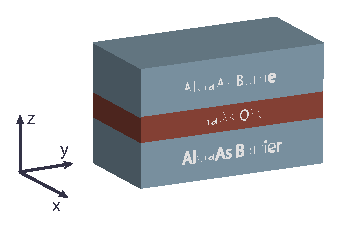
\includegraphics[width = .5\textwidth]{Well.eps}
\caption{sports}
\end{figure}

\section{Quantum Well Disorder}




\section{Microphotoluminescence Spectroscopy}